%% State Space Modelling of Dynamic Systems
%% Lecture 18: General Solution of a State Space System
\def\FileDate{10/02/01}
\def\FileVersion{1.0}
% ----------------------------------------------------------------
% Notes pages *********************************************************
% ----------------------------------------------------------------

In this lecture we conclude our introduction to state space systems by developing a method that can be used to solve any linear time invariant (LTI) system using the state space model. This will put on a formal mathematical footing the approach described in Lecture 15. To do this we need to derive the Taylor series for the state matrix and then use the results from the previous two lectures to formally derive the state transmission matrix $\mathbf{\phi}(t)$ from the resolvant matrix $\mathbf{\Phi}(\lambda) = |\lambda\mathbf{I}-\mathbf{A}|$. This will lead is to a general solution which we will illustrate with examples and compare with the solution developed in the last lecture and the solution obtained by inverting the system transfer function. As before, we will refer to Matlab where relevant.

Once we have completed this material, we will be in a position to move on to look at state-space methods for control system design.

\section*{The Matrix Exponential Function}

In mathematics, the Taylor series is a representation of a function as an infinite sum of terms calculated from the values of its derivatives at a single point. It is named after the English mathematician Brook Taylor. It is common practice to use a finite number of terms of the series to approximate a function. The Taylor series may be regarded as the limit of the Taylor polynomials.\footnote{Definition from `Taylor Series', Wikipedia.}

We use Taylor series to approximate general functions, and here we adapt the Taylor series to discover the form of a function of a matrix.
 

\begin{center}
	\resizebox{200pt}{!}{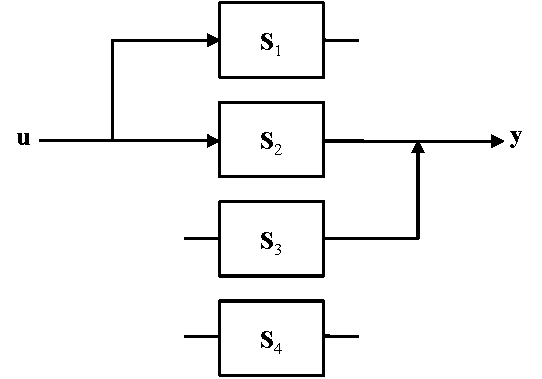
\includegraphics{pictures/partitioning.pdf}}
\end{center}
\endinput

%%% Local Variables: 
%%% mode: latex
%%% TeX-master: "notes"
%%% End:
\ifslidesonly
\begin{slide}
	\heading{Taylor series}
   
\begin{center}
	\resizebox{200pt}{!}{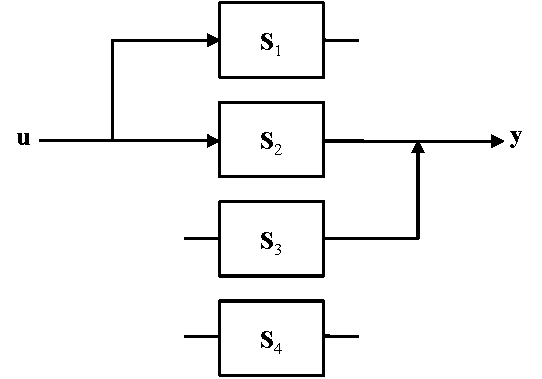
\includegraphics{pictures/partitioning.pdf}}
\end{center}
\endinput

%%% Local Variables: 
%%% mode: latex
%%% TeX-master: "notes"
%%% End:
\end{slide}
\fi

 

Given the transformation $\mathbf{T}^{-1}\mathbf{AT}=\mathbf{\Lambda}$:
\begin{eqnarray*}
	\mathbf{A}t & = & (\mathbf{T\Lambda T}^{-1}) t \\
	\mathbf{A}^nt^n & = & (\mathbf{T\Lambda T}^{-1})(\mathbf{T\Lambda T}^{-1})\ldots(\mathbf{T\Lambda T}^{-1})t^n \\
	                & = & \mathbf{T\Lambda T}^{-1}\mathbf{T\Lambda T}^{-1}\ldots\mathbf{T\Lambda T}^{-1}t^n \\
	\mathbf{A}^nt^n & = & \mathbf{T\Lambda}\mathbf{I}\mathbf{\Lambda I}\ldots\mathbf{I\Lambda T}^{-1}t^n \\
	\               & = & \mathbf{T\Lambda}^n\mathbf{T}^{-1}t^n \\
\end{eqnarray*}
\endinput

%%% Local Variables: 
%%% mode: latex
%%% TeX-master: "notes"
%%% End:
\ifslidesonly
\begin{slide}
	\heading{Using the Similarity Transform}
   Given the transformation $\mathbf{T}^{-1}\mathbf{AT}=\mathbf{\Lambda}$:
\begin{eqnarray*}
	\mathbf{A}t & = & (\mathbf{T\Lambda T}^{-1}) t \\
	\mathbf{A}^nt^n & = & (\mathbf{T\Lambda T}^{-1})(\mathbf{T\Lambda T}^{-1})\ldots(\mathbf{T\Lambda T}^{-1})t^n \\
	                & = & \mathbf{T\Lambda T}^{-1}\mathbf{T\Lambda T}^{-1}\ldots\mathbf{T\Lambda T}^{-1}t^n \\
	\mathbf{A}^nt^n & = & \mathbf{T\Lambda}\mathbf{I}\mathbf{\Lambda I}\ldots\mathbf{I\Lambda T}^{-1}t^n \\
	\               & = & \mathbf{T\Lambda}^n\mathbf{T}^{-1}t^n \\
\end{eqnarray*}
\endinput

%%% Local Variables: 
%%% mode: latex
%%% TeX-master: "notes"
%%% End:
\end{slide}
\fi


 
The matrix function becomes:
\begin{eqnarray*}
	f(\mathbf{A}t) & = & f_0\mathbf{TIT}^{-1} + f_1\mathbf{T\Lambda T}^{-1}t + f_2\mathbf{T\Lambda}^2\mathbf{T}^{-1}t^2 + \cdots + f_n\mathbf{T\Lambda}^n\mathbf{T}^{-1}t^n + \cdots \\
	f(\mathbf{A}t) & = & \mathbf{T}\left(f_0\mathbf{I} + f_1\mathbf{\Lambda}t + f_2\mathbf{\Lambda}^2t^2 + \cdots + f_n\mathbf{\Lambda}^nt^n + \cdots \right)\mathbf{T}^{-1}\\
	               & = & \mathbf{T}f(\mathbf{\Lambda}t)\mathbf{T}^{-1}
\end{eqnarray*}
 
The term inside the brackets on the rhs is a diagonal matrix and the $i^\mathrm{th}$ diagonal element is:
\[
f_0+f_1\lambda_it + f_2\lambda_i^2t^2 + \cdots + f_n\lambda_i^nt^ + \cdots
\]
From the Taylor series this must be $f(\lambda_i t)$:
\[
f(\mathbf{A} t)=\mathbf{T} f(\mathbf{\Lambda} t) \mathbf{T}^{-1}
\]   
where $f(\mathbf{\Lambda} t)=\mathrm{diag}\left(f(\lambda_i t)\right)$.

\endinput

%%% Local Variables: 
%%% mode: latex
%%% TeX-master: "notes"
%%% End:
\ifslidesonly
\begin{slide}
	\heading{Matrix Function}
   The matrix function becomes:
\begin{eqnarray*}
	f(\mathbf{A}t) & = & f_0\mathbf{TIT}^{-1} + f_1\mathbf{T\Lambda T}^{-1}t + f_2\mathbf{T\Lambda}^2\mathbf{T}^{-1}t^2 + \cdots + f_n\mathbf{T\Lambda}^n\mathbf{T}^{-1}t^n + \cdots \\
	f(\mathbf{A}t) & = & \mathbf{T}\left(f_0\mathbf{I} + f_1\mathbf{\Lambda}t + f_2\mathbf{\Lambda}^2t^2 + \cdots + f_n\mathbf{\Lambda}^nt^n + \cdots \right)\mathbf{T}^{-1}\\
	               & = & \mathbf{T}f(\mathbf{\Lambda}t)\mathbf{T}^{-1}
\end{eqnarray*}
 
The term inside the brackets on the rhs is a diagonal matrix and the $i^\mathrm{th}$ diagonal element is:
\[
f_0+f_1\lambda_it + f_2\lambda_i^2t^2 + \cdots + f_n\lambda_i^nt^ + \cdots
\]
From the Taylor series this must be $f(\lambda_i t)$:
\[
f(\mathbf{A} t)=\mathbf{T} f(\mathbf{\Lambda} t) \mathbf{T}^{-1}
\]   
where $f(\mathbf{\Lambda} t)=\mathrm{diag}\left(f(\lambda_i t)\right)$.

\endinput

%%% Local Variables: 
%%% mode: latex
%%% TeX-master: "notes"
%%% End:
\end{slide}
\fi

 
The vector $[v_{31}, i_{1}]^T$ is called the ``\emph{state
vector}.'' Its elements are state variables.
\endinput
%%% Local Variables: 
%%% mode: latex
%%% TeX-master: "notes"
%%% End: 

\ifslidesonly
\begin{slide}
	\heading{Transition Matrix}
   The vector $[v_{31}, i_{1}]^T$ is called the ``\emph{state
vector}.'' Its elements are state variables.
\endinput
%%% Local Variables: 
%%% mode: latex
%%% TeX-master: "notes"
%%% End: 

\end{slide}
\fi


From previous work the error dynamics are:
\[
\dot{\mathbf{e}} = (\mathbf{A}-\mathbf{LC})\mathbf{e}
\]
Therefore the dynamics of the combined system is:
\[\left[ {\begin{array}{*{20}c}
   {\dot{\mathbf{x}}}  \\
   {\dot{\mathbf{e}}ß}  \\
\end{array}} \right] = \left[ {\begin{array}{*{20}c}
   {\left( {{\bf{A}} - {\bf{BK}}} \right)} & {{\bf{BK}}}  \\
   {\bf{0}} & {\left( {{\bf{A}} - {\bf{LC}}} \right)}  \\
\end{array}} \right]\left[ {\begin{array}{*{20}c}
   {\bf{x}}  \\
   {\bf{e}}  \\
\end{array}} \right] + \left[ {\begin{array}{*{20}c}
   {\bf{B}}  \\
   {\bf{0}}  \\
\end{array}} \right]r
\]
\endinput

%%% Local Variables: 
%%% mode: latex
%%% TeX-master: "notes"
%%% End:
\ifslidesonly
\begin{slide}
	\heading{Forced Solution}
   From previous work the error dynamics are:
\[
\dot{\mathbf{e}} = (\mathbf{A}-\mathbf{LC})\mathbf{e}
\]
Therefore the dynamics of the combined system is:
\[\left[ {\begin{array}{*{20}c}
   {\dot{\mathbf{x}}}  \\
   {\dot{\mathbf{e}}ß}  \\
\end{array}} \right] = \left[ {\begin{array}{*{20}c}
   {\left( {{\bf{A}} - {\bf{BK}}} \right)} & {{\bf{BK}}}  \\
   {\bf{0}} & {\left( {{\bf{A}} - {\bf{LC}}} \right)}  \\
\end{array}} \right]\left[ {\begin{array}{*{20}c}
   {\bf{x}}  \\
   {\bf{e}}  \\
\end{array}} \right] + \left[ {\begin{array}{*{20}c}
   {\bf{B}}  \\
   {\bf{0}}  \\
\end{array}} \right]r
\]
\endinput

%%% Local Variables: 
%%% mode: latex
%%% TeX-master: "notes"
%%% End:
\end{slide}
\fi


 
\subsection*{Example 1}

\textbf{Problem}: Find the solution of:
% MathType!MTEF!2!1!+-
% faaagaart1ev2aaaKnaaaaWenf2ys9wBH5garuavP1wzZbqedmvETj
% 2BSbqefm0B1jxALjharqqtubsr4rNCHbGeaGqiVu0Je9sqqrpepC0x
% bbL8FesqqrFfpeea0xe9Lq-Jc9vqaqpepm0xbba9pwe9Q8fs0-yqaq
% pepae9pg0FirpepeKkFr0xfr-xfr-xb9Gqpi0dc9adbaqaaeGaciGa
% aiaabeqaamaabaabaaGcbaWaaSaaaeaacaWGKbGaaCiEaaqaaiaads
% gacaWG0baaaiabg2da9maadmaabaqbamqabiGaaaqaaiabgkHiTiaa
% iodaaeaacqGHsislcaaIYaaabaGaaGymaaqaaiaaicdaaaaacaGLBb
% GaayzxaaGaaCiEaiabgUcaRmaadmaabaqbamqabiqaaaqaaiaaigda
% aeaacaaIWaaaaaGaay5waiaaw2faaiaadwhaaaa!4013!
\[
\frac{{d{\bf{x}}}}{{dt}} = \left[ {\begin{array}{*{20}c}
   { - 3} & { - 2}  \\
   1 & 0  \\
\end{array}} \right]{\bf{x}} + \left[ {\begin{array}{*{20}c}
   1  \\
   0  \\
\end{array}} \right]u
\]
given $\mathbf{x}_0=[1,\ 1]^T$, and $u = 1$ for $t\ge 0$.

\textbf{SOLUTION}: The state matrix $\mathbf{A}$ is the same as Example 4 from Lecture 17, so the transformation matrix is:
% MathType!MTEF!2!1!+-
% faaagaart1ev2aaaKnaaaaWenf2ys9wBH5garuavP1wzZbqedmvETj
% 2BSbqefm0B1jxALjharqqtubsr4rNCHbGeaGqiVu0Je9sqqrpepC0x
% bbL8FesqqrFfpeea0xe9Lq-Jc9vqaqpepm0xbba9pwe9Q8fs0-yqaq
% pepae9pg0FirpepeKkFr0xfr-xfr-xb9Gqpi0dc9adbaqaaeGaciGa
% aiaabeqaamaabaabaaGcbaGaaCivaiabg2da9iabg2da9maadmaaba
% qbamqabiGaaaqaaiaaigdaaeaacaaIXaaabaGaeyOeI0IaaGymaaqa
% aiabgkHiTiaaicdacaGGUaGaaGynaaaaaiaawUfacaGLDbaaaaa!3935!
\[
{\bf{T}} = \left[ {\begin{array}{*{20}c}
   1 & 1  \\
   { - 1} & { - 0.5}  \\
\end{array}} \right]
\]
with an inverse:
% MathType!MTEF!2!1!+-
% faaagaart1ev2aaaKnaaaaWenf2ys9wBH5garuavP1wzZbqedmvETj
% 2BSbqefm0B1jxALjharqqtubsr4rNCHbGeaGqiVu0Je9sqqrpepC0x
% bbL8FesqqrFfpeea0xe9Lq-Jc9vqaqpepm0xbba9pwe9Q8fs0-yqaq
% pepae9pg0FirpepeKkFr0xfr-xfr-xb9Gqpi0dc9adbaqaaeGaciGa
% aiaabeqaamaabaabaaGcbaGaaCivamaaCaaaleqabaGaeyOeI0IaaG
% ymaaaakiabg2da9iabg2da9maadmaabaqbamqabiGaaaqaaiabgkHi
% TiaaigdaaeaacqGHsislcaaIYaaabaGaaGOmaaqaaiaaikdaaaaaca
% GLBbGaayzxaaaaaa!39A7!
\[
{\bf{T}}^{ - 1}  = \left[ {\begin{array}{*{20}c}
   { - 1} & { - 2}  \\
   2 & 2  \\
\end{array}} \right]
\]
and with corresponding eigenvalues $\lambda_1=-1$ and $\lambda_2=-2$.
 
Therefore the state transition matrix is:
\begin{eqnarray*}
\mathbf{\phi}(t) & = & e^{\mathbf{A}t}=\mathbf{T}e^{\mathbf{\Lambda}t}\mathbf{T}^{-1} \\
	             & = & \left[ {\begin{array}{*{20}c}
	   1 & 1  \\
	   { - 1} & { - 0.5}  \\
	\end{array}} \right]\left[ {\begin{array}{*{20}c}
	   {e^{ - t} } & 0  \\
	   0 & {e^{ - 2t} }  \\
	\end{array}} \right]\left[ {\begin{array}{*{20}c}
	   { - 1} & { - 2}  \\
	   2 & 2  \\
	\end{array}} \right] \\
	             & = & \left[ {\begin{array}{*{20}c}
	   1 & 1  \\
	   { - 1} & { - 0.5}  \\
	\end{array}} \right]\left[ {\begin{array}{*{20}c}
	   {-e^{ - t} } & {-2e^{ - t} }  \\
	   {2e^{ - 2t} } & {2e^{ - 2t} }  \\
	\end{array}} \right] \\
	             & = & \left[ {\begin{array}{*{20}c}
	   \left\{ {-e^{ - t} + 2e^{-2t}} \right\} & \left\{ {-2e^{ - t} + 2e^{-2t}} \right\}  \\
	   \left\{ {e^{ - t} - e^{-2t}} \right\} & \left\{ {2e^{ - t} - e^{-2t}} \right\}  \\
	\end{array}} \right] \\
\end{eqnarray*}

 
The solution is:
\[
\mathbf{x}(t) = \mathrm{term}_1+\int_0^t\mathrm{term}_2 d\tau.
\]
where $\mathrm{term}_1=\mathbf{\phi}(t)\mathbf{x}_0=e^{\mathbf{A}t}\mathbf{x}_0$.
\begin{eqnarray*}
\mathrm{term}_1 & = & \left[ {\begin{array}{*{20}c}
	   \left\{ {-e^{ - t} + 2e^{-2t}} \right\} & \left\{ {-2e^{ - t} + 2e^{-2t}} \right\}  \\
	   \left\{ {e^{ - t} - e^{-2t}} \right\} & \left\{ {2e^{ - t} - e^{-2t}} \right\}  \\
	\end{array}} \right] \left[ {\begin{array}{*{20}c}
	   1  \\
	   1  \\
	\end{array}} \right] \\
	& = & \left[ {\begin{array}{*{20}c}
	   {\left\{ {\left. { - 3e^{ - t}  + 4e^{ - 2t} } \right\}} \right.}  \\
	   {\left\{ {\left. {3e^{ - t}  - 2e^{ - 2t} } \right\}} \right.}  \\
	\end{array}} \right]
\end{eqnarray*}
and
\begin{eqnarray*}
	{\rm{term}}_2  & = & e^{{\bf{A}}(t - \tau )} {\bf{B}}u = e^{{\bf{A}}(t - \tau )} \left[ {\begin{array}{*{20}c}
	   1  \\
	   0  \\
	\end{array}} \right] \times 1 \\
 & = & \left[ {\begin{array}{*{20}c}
   {\left. {\left\{ { - e^{ - (t - \tau )}  + 2e^{ - 2(t - \tau )} } \right.} \right\}}  \\
   {\left. {\left\{ {e^{ - (t - \tau )}  - e^{ - 2(t - \tau )} } \right.} \right\}}  \\
\end{array}} \right]
\end{eqnarray*}

\begin{eqnarray*}
	\int_0^t {{\rm{term}}_2 d\tau }  & = & \left[ {\begin{array}{*{20}c}
	   {\int_0^t {\left. {\left\{ { - e^{ - (t - \tau )}  + 2e^{ - 2(t - \tau )} } \right.} \right\}d\tau } }  \\
	   {\int_0^t {\left. {\left\{ {e^{ - (t - \tau )}  - e^{ - 2(t - \tau )} } \right.} \right\}d\tau } }  \\
	\end{array}} \right] \\
	& = & 
	  \left[ {\begin{array}{*{20}c}
	   {\left. {\left\{ { - e^{ - (t - \tau )}  + e^{ - 2(t - \tau )} } \right.} \right\}}  \\
	   {\left. {\left\{ {e^{ - (t - \tau )}  - 0.5e^{ - 2(t - \tau )} } \right.} \right\}}  \\
	\end{array}} \right]_{\tau  = 0}^t  \\ 
	 & = & \left[ {\begin{array}{*{20}c}
	   { - 1 + e^{ - t}  + 1 - e^{ - 2t} }  \\
	   { - 1 + e^{ - t}  - 0.5 + 0.5e^{ - 2t} }  \\
	\end{array}} \right] \\ 
	 &  = & \left[ {\begin{array}{*{20}c}
	   {e^{ - t}  - e^{ - 2t} }  \\
	   {0.5 - e^{ - t}  + 0.5e^{ - 2t} }  \\
	\end{array}} \right]
\end{eqnarray*}

Combining $\mathrm{term}_1$ and $\int_0^t \mathrm{term}_2 d\tau$ we find the total, forced, response:
\[
{\bf{x}}(t) = \left[ {\begin{array}{*{20}c}
   { - 3e^{ - t}  + 4e^{ - 2t} }  \\
   {3e^{ - t}  - 2e^{ - 2t} }  \\
\end{array}} \right] + \left[ {\begin{array}{*{20}c}
   {e^{ - t}  - e^{ - 2t} }  \\
   {0.5 - e^{ - t}  + 0.5e^{ - 2t} }  \\
\end{array}} \right]
\]

Therefore:
% MathType!MTEF!2!1!+-
% faaagaart1ev2aaaKnaaaaWenf2ys9wBH5garuavP1wzZbqedmvETj
% 2BSbqefm0B1jxALjharqqtubsr4rNCHbGeaGqiVu0Je9sqqrpepC0x
% bbL8FesqqrFfpeea0xe9Lq-Jc9vqaqpepm0xbba9pwe9Q8fs0-yqaq
% pepae9pg0FirpepeKkFr0xfr-xfr-xb9Gqpi0dc9adbaqaaeGaciGa
% aiaabeqaamaabaabaaGcbaGaaCiEaiaacIcacaWG0bGaaiykaiabg2
% da9maadmaabaqbamqabiqaaaqaaiabgkHiTiaaikdacaWGLbWaaWba
% aSqabeaacqGHsislcaWG0baaaOGaey4kaSIaaG4maiaadwgadaahaa
% WcbeqaaiabgkHiTiaaikdacaWG0baaaaGcbaGaaGimaiaac6cacaaI
% 1aGaey4kaSIaaGOmaiaadwgadaahaaWcbeqaaiabgkHiTiaadshaaa
% GccqGHsislcaaIXaGaaiOlaiaaiwdacaWGLbWaaWbaaSqabeaacqGH
% sislcaaIYaGaamiDaaaaaaaakiaawUfacaGLDbaaaaa!4C2A!
\[
{\bf{x}}(dt) = \left[ {\begin{array}{*{20}c}
   { - 2e^{ - t}  + 3e^{ - 2t} }  \\
   {0.5 + 2e^{ - t}  - 1.5e^{ - 2t} }  \\
\end{array}} \right]
\]


 

\subsection*{Alternative solution 1}
Using the transformation to normal canonical form:
\[
\frac{d\mathbf{w}}{t}=\mathbf{\Lambda w}+ \mathbf{T}^{-1}\mathbf{B}u
\]
% MathType!MTEF!2!1!+-
% faaagaart1ev2aaaKnaaaaWenf2ys9wBH5garuavP1wzZbqedmvETj
% 2BSbqefm0B1jxALjharqqtubsr4rNCHbGeaGqiVu0Je9sqqrpepC0x
% bbL8FesqqrFfpeea0xe9Lq-Jc9vqaqpepm0xbba9pwe9Q8fs0-yqaq
% pepae9pg0FirpepeKkFr0xfr-xfr-xb9Gqpi0dc9adbaqaaeGaciGa
% aiaabeqaamaabaabaaGcbaWaaSaaaeaacaWGKbGaaC4Daaqaaiaads
% gacaWG0baaaiabg2da9maadmaabaqbamqabiGaaaqaaiabgkHiTiaa
% igdaaeaacaaIWaaabaGaaGimaaqaaiabgkHiTiaaikdaaaaacaGLBb
% GaayzxaaGaaC4DaiabgUcaRmaadmaabaqbamqabiGaaaqaaiabgkHi
% TiaaigdaaeaacqGHsislcaaIYaaabaGaaGOmaaqaaiaaikdaaaaaca
% GLBbGaayzxaaWaamWaaeaafaWabeGabaaabaGaaGymaaqaaiaaicda
% aaaacaGLBbGaayzxaaGaamyDaiaacUdacaaMf8UaamyDaiabg2da9i
% aaigdaaaa!4BE3!
\[
\frac{{d{\bf{w}}}}{{dt}} = \left[ {\begin{array}{*{20}c}
   { - 1} & 0  \\
   0 & { - 2}  \\
\end{array}} \right]{\bf{w}} + \left[ {\begin{array}{*{20}c}
   { - 1} & { - 2}  \\
   2 & 2  \\
\end{array}} \right]\left[ {\begin{array}{*{20}c}
   1  \\
   0  \\
\end{array}} \right]u;\quad u = 1
\]
\[
\frac{dw_1}{dt}=-w_1-1\ \textrm{and}\ \frac{dw_2}{dt}=-2w_2 + 2
\]
% MathType!MTEF!2!1!+-
% faaagaart1ev2aaaKnaaaaWenf2ys9wBH5garuavP1wzZbqedmvETj
% 2BSbqefm0B1jxALjharqqtubsr4rNCHbGeaGqiVu0Je9sqqrpepC0x
% bbL8FesqqrFfpeea0xe9Lq-Jc9vqaqpepm0xbba9pwe9Q8fs0-yqaq
% pepae9pg0FirpepeKkFr0xfr-xfr-xb9Gqpi0dc9adbaqaaeGaciGa
% aiaabeqaamaabaabaaGcbaGaaC4DamaaBaaaleaacaaIWaaabeaaki
% abg2da9iaahsfadaahaaWcbeqaaiabgkHiTiaaigdaaaGccaWH4bWa
% aSbaaSqaaiaaicdaaeqaaOGaeyypa0ZaamWaaeaafaWabeGacaaaba
% GaeyOeI0IaaGymaaqaaiabgkHiTiaaikdaaeaacaaIYaaabaGaaGOm
% aaaaaiaawUfacaGLDbaadaWadaqaauaadeqaceaaaeaacaaIXaaaba
% GaaGymaaaaaiaawUfacaGLDbaacqGH9aqpdaWadaqaauaadeqaceaa
% aeaacqGHsislcaaIZaaabaGaaGinaaaaaiaawUfacaGLDbaaaaa!466E!
\[
{\bf{w}}_0  = {\bf{T}}^{ - 1} {\bf{x}}_0  = \left[ {\begin{array}{*{20}c}
   { - 1} & { - 2}  \\
   2 & 2  \\
\end{array}} \right]\left[ {\begin{array}{*{20}c}
   1  \\
   1  \\
\end{array}} \right] = \left[ {\begin{array}{*{20}c}
   { - 3}  \\
   4  \\
\end{array}} \right]
\]


\begin{eqnarray*}
	w_1 & = & w_{10}e^{-t}-\int_0^t e^{-(t-\tau)} d\tau \\
	    & = & -3e^{-t}-\left[e^{-(t-\tau)}\right]_0^t \\
	    & = & -3e^{-t}-\left[1 - e^{-t}\right] \\
	    & = & -1 -2e^{-t}	
\end{eqnarray*}
 
\begin{eqnarray*}
	w_2 & = & w_{20}e^{-2t}+2\int_0^t e^{-2(t-\tau)} d\tau \\
	    & = & 4e^{-2t}+2\left[0.5e^{-2(t-\tau)}\right]_0^t \\
	    & = & 4e^{-2t}+\left[1 - e^{-2t}\right] \\
	    & = & 1 + 3e^{-2t}	
\end{eqnarray*}

% MathType!MTEF!2!1!+-
% faaagaart1ev2aaaKnaaaaWenf2ys9wBH5garuavP1wzZbqedmvETj
% 2BSbqefm0B1jxALjharqqtubsr4rNCHbGeaGqiVu0Je9sqqrpepC0x
% bbL8FesqqrFfpeea0xe9Lq-Jc9vqaqpepm0xbba9pwe9Q8fs0-yqaq
% pepae9pg0FirpepeKkFr0xfr-xfr-xb9Gqpi0dc9adbaqaaeGaciGa
% aiaabeqaamaabaabaaGcbaGaaCiEaiabg2da9iaahsfacaWH3bGaey
% ypa0ZaamWaaeaafaWabeGacaaabaGaaGymaaqaaiaaigdaaeaacqGH
% sislcaaIXaaabaGaeyOeI0IaaGimaiaac6cacaaI1aaaaaGaay5wai
% aaw2faamaadmaabaqbamqabiqaaaqaaiabgkHiTiaaigdacqGHsisl
% caaIYaGaamyzamaaCaaaleqabaGaeyOeI0IaamiDaaaaaOqaaiaaig
% dacqGHRaWkcaaIZaGaamyzamaaCaaaleqabaGaeyOeI0IaaGOmaiaa
% dshaaaaaaaGccaGLBbGaayzxaaaaaa!49AC!
\[
{\bf{x}} = {\bf{Tw}} = \left[ {\begin{array}{*{20}c}
   1 & 1  \\
   { - 1} & { - 0.5}  \\
\end{array}} \right]\left[ {\begin{array}{*{20}c}
   { - 1 - 2e^{ - t} }  \\
   {1 + 3e^{ - 2t} }  \\
\end{array}} \right]
\]
Therefore
% MathType!MTEF!2!1!+-
% faaagaart1ev2aaaKnaaaaWenf2ys9wBH5garuavP1wzZbqedmvETj
% 2BSbqefm0B1jxALjharqqtubsr4rNCHbGeaGqiVu0Je9sqqrpepC0x
% bbL8FesqqrFfpeea0xe9Lq-Jc9vqaqpepm0xbba9pwe9Q8fs0-yqaq
% pepae9pg0FirpepeKkFr0xfr-xfr-xb9Gqpi0dc9adbaqaaeGaciGa
% aiaabeqaamaabaabaaGcbaGaaCiEaiabg2da9maadmaabaqbamqabi
% qaaaqaaiabgkHiTiaaikdacaWGLbWaaWbaaSqabeaacqGHsislcaWG
% 0baaaOGaey4kaSIaaG4maiaadwgadaahaaWcbeqaaiabgkHiTiaaik
% dacaWG0baaaaGcbaGaaGimaiaac6cacaaI1aGaey4kaSIaaGOmaiaa
% dwgadaahaaWcbeqaaiabgkHiTiaadshaaaGccqGHsislcaaIXaGaai
% OlaiaaiwdacaWGLbWaaWbaaSqabeaacqGHsislcaaIYaGaamiDaaaa
% aaaakiaawUfacaGLDbaaaaa!49D8!
\[
{\bf{x}} = \left[ {\begin{array}{*{20}c}
   { - 2e^{ - t}  + 3e^{ - 2t} }  \\
   {0.5 + 2e^{ - t}  - 1.5e^{ - 2t} }  \\
\end{array}} \right]
\]


 
\subsection*{Alternative solution 2} 
Using the Laplace transform method.

Taking Laplace transforms of the state equations, taking account of the initial conditions:
\[
s\mathbf{X}(s)-\mathbf{x}_0=\mathbf{A}\mathbf{X}(s)+\mathbf{B}U(s)
\]
% MathType!MTEF!2!1!+-
% faaagaart1ev2aaaKnaaaaWenf2ys9wBH5garuavP1wzZbqedmvETj
% 2BSbqefm0B1jxALjharqqtubsr4rNCHbGeaGqiVu0Je9sqqrpepC0x
% bbL8FesqqrFfpeea0xe9Lq-Jc9vqaqpepm0xbba9pwe9Q8fs0-yqaq
% pepae9pg0FirpepeKkFr0xfr-xfr-xb9Gqpi0dc9adbaqaaeGaciGa
% aiaabeqaamaabaabaaGcbaGaaiikaiaadohacaWHjbGaeyOeI0IaaC
% yqaiaacMcacaWHybGaaiikaiaadohacaGGPaGaeyypa0JaaCiEamaa
% BaaaleaacaaIWaaabeaakiabgUcaRiaahkeacaWGvbGaaiikaiaado
% hacaGGPaGaeyypa0ZaamWaaeaafaWabeGabaaabaGaaGymaaqaaiaa
% igdaaaaacaGLBbGaayzxaaGaey4kaSYaamWaaeaafaWabeGabaaaba
% GaaGymaaqaaiaaicdaaaaacaGLBbGaayzxaaWaaSaaaeaacaaIXaaa
% baGaam4Caaaaaaa!4885!
\[
(s{\bf{I}} - {\bf{A}}){\bf{X}}(s) = {\bf{x}}_0  + {\bf{B}}U(s) = \left[ {\begin{array}{*{20}c}
   1  \\
   1  \\
\end{array}} \right] + \left[ {\begin{array}{*{20}c}
   1  \\
   0  \\
\end{array}} \right]\frac{1}{s}
\]
Therefore
% MathType!MTEF!2!1!+-
% faaagaart1ev2aaaKnaaaaWenf2ys9wBH5garuavP1wzZbqedmvETj
% 2BSbqefm0B1jxALjharqqtubsr4rNCHbGeaGqiVu0Je9sqqrpepC0x
% bbL8FesqqrFfpeea0xe9Lq-Jc9vqaqpepm0xbba9pwe9Q8fs0-yqaq
% pepae9pg0FirpepeKkFr0xfr-xfr-xb9Gqpi0dc9adbaqaaeGaciGa
% aiaabeqaamaabaabaaGcbaGaaCiwaiaacIcacaWGZbGaaiykaiabg2
% da9iaacIcacaWGZbGaaCysaiabgkHiTiaahgeacaGGPaWaaWbaaSqa
% beaacqGHsislcaaIXaaaaOWaamWaaeaafaWabeGabaaabaGaaGymai
% abgUcaRmaalaaabaGaaGymaaqaaiaadohaaaaabaGaaGymaaaaaiaa
% wUfacaGLDbaaaaa!3F1F!
\[
{\bf{X}}(s) = (s{\bf{I}} - {\bf{A}})^{ - 1} \left[ {\begin{array}{*{20}c}
   {1 + \frac{1}{s}}  \\
   1  \\
\end{array}} \right]
\]

% MathType!MTEF!2!1!+-
% faaagaart1ev2aaaKnaaaaWenf2ys9wBH5garuavP1wzZbqedmvETj
% 2BSbqefm0B1jxALjharqqtubsr4rNCHbGeaGqiVu0Je9sqqrpepC0x
% bbL8FesqqrFfpeea0xe9Lq-Jc9vqaqpepm0xbba9pwe9Q8fs0-yqaq
% pepae9pg0FirpepeKkFr0xfr-xfr-xb9Gqpi0dc9adbaqaaeGaciGa
% aiaabeqaamaabaabaaGcbaGaaeOtaiaab+gacaqG3bGaaeiiaiaacI
% cacaWGZbGaaCysaiabgkHiTiaahgeacaGGPaWaaWbaaSqabeaacqGH
% sislcaaIXaaaaOGaeyypa0ZaamWaaeaafaWabeGacaaabaGaam4Cai
% abgUcaRiaaiodaaeaacaaIYaaabaGaeyOeI0IaaGymaaqaaiaadoha
% aaaacaGLBbGaayzxaaWaaWbaaSqabeaacqGHsislcaaIXaaaaOGaey
% ypa0ZaaSaaaeaacaaIXaaabaGaaiikaiaadohacqGHRaWkcaaIZaGa
% aiykaiaadohacqGHRaWkcaaIYaaaamaadmaabaqbamqabiGaaaqaai
% aadohaaeaacqGHsislcaaIYaaabaGaaGymaaqaaiaadohacqGHRaWk
% caaIZaaaaaGaay5waiaaw2faaaaa!5355!
\[
{\rm{Now }}(s{\bf{I}} - {\bf{A}})^{ - 1}  = \left[ {\begin{array}{*{20}c}
   {s + 3} & 2  \\
   { - 1} & s  \\
\end{array}} \right]^{ - 1}  = \frac{1}{{(s + 3)s + 2}}\left[ {\begin{array}{*{20}c}
   s & { - 2}  \\
   1 & {s + 3}  \\
\end{array}} \right]
\]
Therefore
\begin{eqnarray*}
	{\bf{X}}(s) & = & \frac{1}{{s^2  + 3s + 2}}\left[ {\begin{array}{*{20}c}
	   s & { - 2}  \\
	   1 & {s + 3}  \\
	\end{array}} \right]\left[ {\begin{array}{*{20}c}
	   {1 + \frac{1}{s}}  \\
	   1  \\
	\end{array}} \right] \\
	            & = & \frac{1}{{(s + 1)(s + 2)}}\left[ {\begin{array}{*{20}c}
	   {s - 1}  \\
	   {\frac{{s^2  + 4s + 1}}{s}}  \\
	\end{array}} \right] \\
	&  = & \left[ {\begin{array}{*{20}c}
	   {\frac{{s - 1}}{{(s + 1)(s + 2)}}}  \\
	   {\frac{{s^2  + 4s + 1}}{{s(s + 1)(s + 2)}}}  \\
	\end{array}} \right]
\end{eqnarray*}

Taking partial fractions:
\[
{\bf{X}}(s) = \left[ {\begin{array}{*{20}c}
   {\frac{{ - 2}}{{s + 1}} + \frac{3}{{s + 2}}}  \\
   {\frac{{0.5}}{s} + \frac{2}{{s + 1}} + \frac{{ - 1.5}}{{s + 2}}}  \\
\end{array}} \right]
\]

Finally, taking inverse Laplace transforms:
\[
{\bf{x}}(t) = \left[ {\begin{array}{*{20}c}
   { - 2e^{ - t}  + 3e^{ - 2t} }  \\
   {0.5 + 2e^{ - t}  - 1.5e^{ - 2t} }  \\
\end{array}} \right]
\]





%----------------------------------------------------------------
% The end of notes
% ----------------------------------------------------------------
\endinput

%%% Local Variables: 
%%% mode: latex
%%% TeX-master: t
%%% End: 
